\documentclass[12pt,a4paper]{article}
\usepackage[a4paper, left=2.5cm,right=2.5cm,top=3cm,bottom=3cm]{geometry}
\usepackage[utf8]{inputenc}
\usepackage[spanish]{babel}
\addto\captionsspanish{
	\renewcommand\chaptername{}
	\renewcommand\appendixname{Anexo}
	\renewcommand\appendixpagename{Anexos}
	\def\tablename{Tabla}
	\def\listtablename{\'Indice de tablas}
}
\usepackage{ucs}
\usepackage{subfig}
\usepackage{float}
\usepackage{amsmath}
\usepackage{amsfonts}
\usepackage{amssymb}
\usepackage{graphicx}
\usepackage{listings}
\usepackage{color}
\usepackage[T1]{fontenc}
\usepackage[scaled]{beramono}
\usepackage{upquote}
\usepackage{xcolor}
\usepackage{listings}
\usepackage{caption}
\usepackage{chngcntr}
\usepackage{endnotes}
\usepackage{float}
\usepackage{hyperref}
\usepackage{wrapfig}
\usepackage{fancyhdr}
\usepackage{emptypage}
\usepackage{times}
\usepackage{array}
\usepackage{setspace}
\usepackage{multirow}
%\usepackage{subfigure}
\usepackage{verbatim}
%\usepackage{tabulary}
%\usepackage{graphicx,subfigure}
\usepackage[bottom]{footmisc} 
\usepackage{appendix}
\usepackage{mathtools}
\usepackage{textcomp}


%listing, code style
% Define a custom color
\definecolor{backcolour}{rgb}{0.95,0.95,0.92}
\definecolor{codegreen}{rgb}{0,0.6,0}

% Define listing style
\lstset{
	language=python,
	tabsize=4,
	rulecolor=,
	basicstyle=\scriptsize,
	upquote=true,
	aboveskip={1.2\baselineskip},
	columns=fixed,
	numbers=left,
	showstringspaces=false,
	extendedchars=true,
	breaklines=true,
	prebreak = \raisebox{0ex}[0ex][0ex]{\ensuremath{\hookleftarrow}},
	showtabs=false,
	showspaces=false,
	showstringspaces=false,
	identifierstyle=\ttfamily,
	keywordstyle=\color[rgb]{0,0,1},
	commentstyle=\color[rgb]{0.133,0.545,0.133},
	stringstyle=\color[rgb]{0.627,0.126,0.941},
} 


\renewcommand{\notesname}{Fuentes}
\renewcommand{\baselinestretch}{1.2}
\hypersetup{
	colorlinks,%
	citecolor=black,%
	filecolor=black,%
	linkcolor=black,%
	urlcolor=black
}

\begin{document}
	
\begin{titlepage}
	\centering
	%\null\vfill
	
\includegraphics[width=\textwidth]{FIGURES/Portada/Logo_portada.png} 
	\vspace{1.5cm}
	
	Universidad Politécnica de Madrid
	\\Escuela Técnica Superior de Ingeniería Aeronáutica y del Espacio
	\vspace{2cm}
	
	{\large MÁSTER UNIVERSITARIO EN SISTEMAS ESPACIALES}
	\vspace{2cm}
	
	{\LARGE MILESTONE 2}
	\vspace{1cm}
	
	{\large Ampliación de Matemáticas I}
	\vspace{4cm}
	
	\begin{center}
		\large{\textbf{\today}} \\
	\end{center}
	
	Autor: \\ Alberto García Rincón
	\vfill
\end{titlepage}

%****INDICES****
\newpage
\pagestyle{empty}
\tableofcontents	

%******DOC******	
\newpage
\pagenumbering{arabic}
\setcounter{page}{1}
\pagestyle{fancy} 

\section{Introducción}
Como continuación del ejercicio resuelto durante la semana anterior, se ha reestructurado el código referente al programa para resolver el problema de Cauchy aplicado para la resolución de una órbita Kepleriana mediante distintos métodos. Aparte de resolver el problema con el método explícito de Euler y con el método de Runge-Kutta de cuarto orden, que ya se programaron para el anterior ejercicio, se han añadido los métodos de Euler implícito y el método de Crank-Nicolson.

Se procederá a una explicación del código usado para la resolución de este ejercicio y a un breve análisis de los resultados obtenidos.

\section{Código de Python}
Para este ejercicio se ha procedido a una separación del programa principal o $"main"$ (denominado \textit{Milestone\_2.py}) donde se llaman a los distintos procesos o funciones que se encuentran en otros archivos individuales.

\subsection{\textit{Milestone\_2.py}}
El programa principal contiene las condiciones iniciales del problema a resolver y va llamando a los distintos subprogramas o funciones para obtener los distintos resultados según el método que se use. Por tanto en el programa $"main"$ se tienen todos los datos calculados de los distintos métodos que aquí se implementan. Estos datos se almacenan en una variable, la cual se pasa como argumento a las funciones encargadas de dibujar las gráficas que se encuentran definidas en otro archivo distinto.
\begin{figure}[H] 
	\centering
	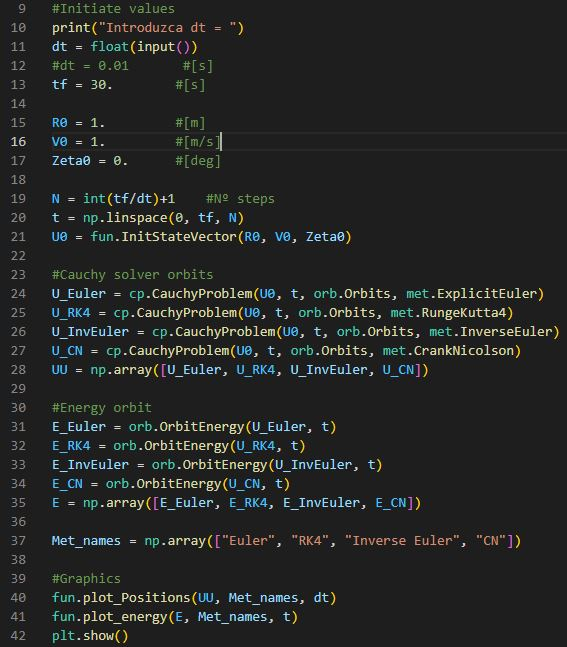
\includegraphics[width=0.8\textwidth]{FIGURES/Codigo/main.jpg}
	\caption{\textit{Milestone\_2.py}.}
\end{figure}

\subsection{\textit{CauchyProblem.py}}
En otro archivo se tiene programado el problema de Cauchy, al cual se le llama desde el $main$ y se le aporta como argumentos las condiciones iniciales, el tiempo de simulación, la función que define la órbita (la cuál está programada en otro archivo distinto denominado  \textit{Orbits.py}) y el método que se usa para la resolución (estos métodos están programados en otro archivo: \textit{Methods.py}). 

Este código itera el numero de repeticiones definido como la división entre el tiempo total de la simulación y el intervalo de tiempo de discretización.
\begin{figure}[H] 
	\centering
	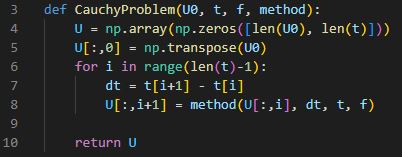
\includegraphics[width=0.6\textwidth]{FIGURES/Codigo/CauchyProblem.jpg}
	\caption{\textit{CauchyProblem.py}.}
\end{figure}

\subsection{\textit{Methods.py}}
A continuación se muestra el código de los distintos métodos de cálculo que se utilizan. 

Cabe destacar que para el método de Euler inverso y para el método de Crank-Nicolson, al tratarse de métodos implícitos se ha usado el método de $newton$ de la librería de Python $scipy.optimize$. En el caso del método de Euler inverso ha sido necesario la configuración de la tolerancia ($tol$) en la resolución e indicar el número máximo de interacciones del método para obtener el resultado ($maxiter$) , de lo contrario la función no conseguía llegar a una solución para determinadas condiciones iniciales ($\Delta t \geq 0.1 s$).
\begin{figure}[H] 
	\centering
	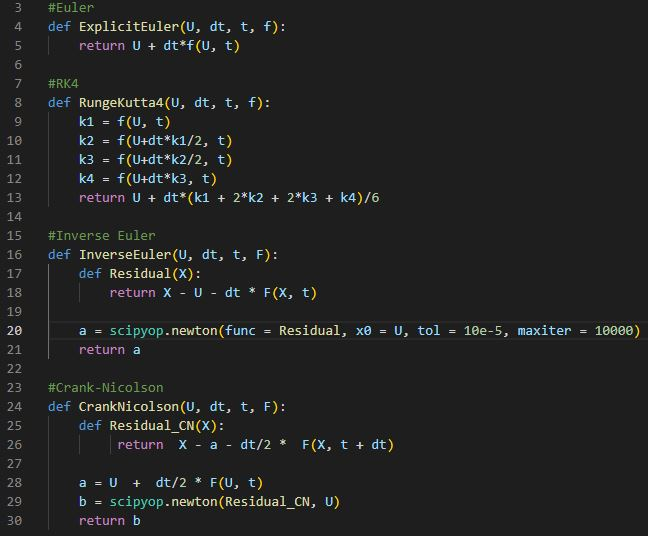
\includegraphics[width=0.8\textwidth]{FIGURES/Codigo/methods.jpg}
	\caption{\textit{Methods.py}.}
\end{figure}

\subsection{\textit{Orbits.py}}
En el siguiente archivo de ha programado la función que define la órbita de Kepler. También se ha programado una función que calcula la energía específica de la órbita, esto nos servirá para analizar el comportamiento de las órbitas calculadas a través de los distintos métodos y compararlos entre sí.
\begin{figure}[H] 
	\centering
	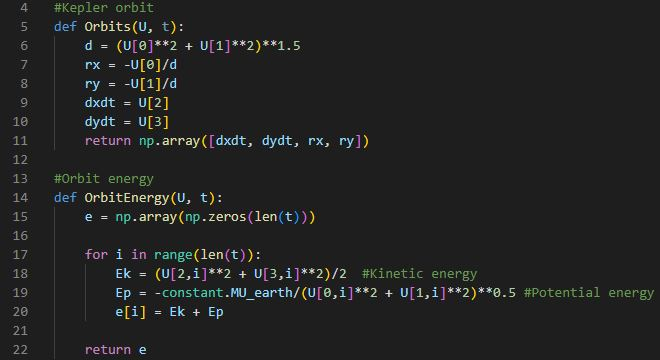
\includegraphics[width=0.8\textwidth]{FIGURES/Codigo/orbits.jpg}
	\caption{\textit{Orbits.py}.}
\end{figure}

\subsection{\textit{Constant.py}}
Se han definido unas constantes en otro archivo. Estas constantes son utilizadas por algunas funciones del programa. 
\begin{figure}[H] 
	\centering
	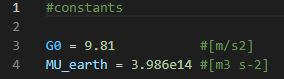
\includegraphics[width=0.5\textwidth]{FIGURES/Codigo/constants.jpg}
	\caption{\textit{constant.py}.}
\end{figure}

\subsection{\textit{Functions.py}}
Por último se ha creado otro archivo con el resto de funciones: función para inicializar el vector de estado; funciones para dibujar la posición de la órbita según ejes X e Y y función para graficar la energía específica en función del tiempo.
\begin{figure}[H] 
	\centering
	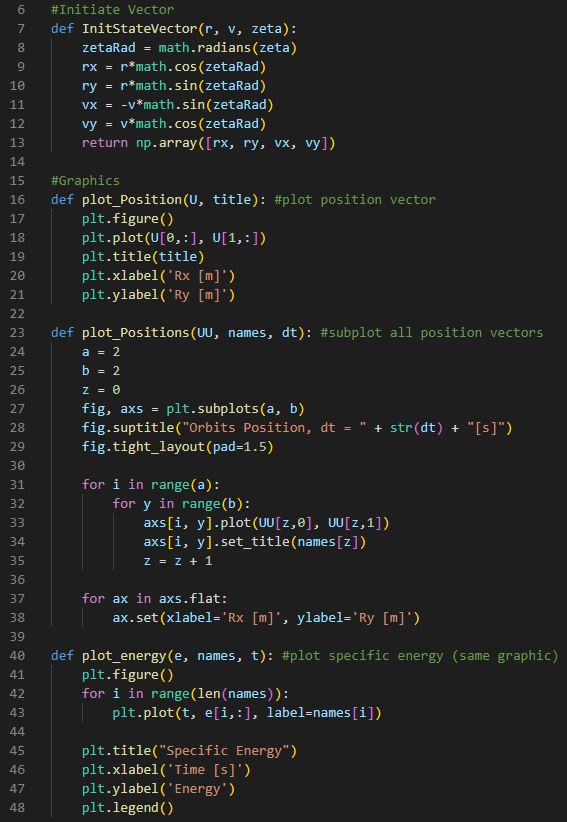
\includegraphics[width=0.8\textwidth]{FIGURES/Codigo/functions.jpg}
	\caption{\textit{Functions.py}.}
\end{figure} 


\section{Resultados de los métodos}
Se ha fijado un tiempo total de simulación de 30 segundos se han realizado varias simulaciones con distintos $\Delta t$ para comprobar que el código funciona correctamente. Aquí solo se muestran algunas de esas simulaciones.
%Aquí solo se muestran los resultados con $\Delta t = 0.001 s$ utilizando las función $newton$ de la librería de Python $scipy.optimize$.

\subsection{Simulaciones con: $\Delta t = 0.1 s$}
Los métodos de Runge-Kutta y Crank-Nicolson no acumulan apenas error respecto a la resolución analítica durante el tiempo de simulación. Esto queda reflejado en la energía específica obtenida con estos métodos se mantiene constante durante toda la simulación. 

Sin embargo el método de Euler explícito va aumentando su energía, lo que se traduce en que el objeto que simulamos en la órbita se aleja cada vez más, formando una espiral. 

En el método de Euler inverso ocurre que la energía disminuye durante los primeros 3 segundos, lo que quiere decir que el objeto se acerca cada vez más al origen de coordenadas, hasta que converge en dicho punto y comienza aumentar la energía obteniéndose un resultado no válido.  
\begin{figure}[H] 
	\centering
	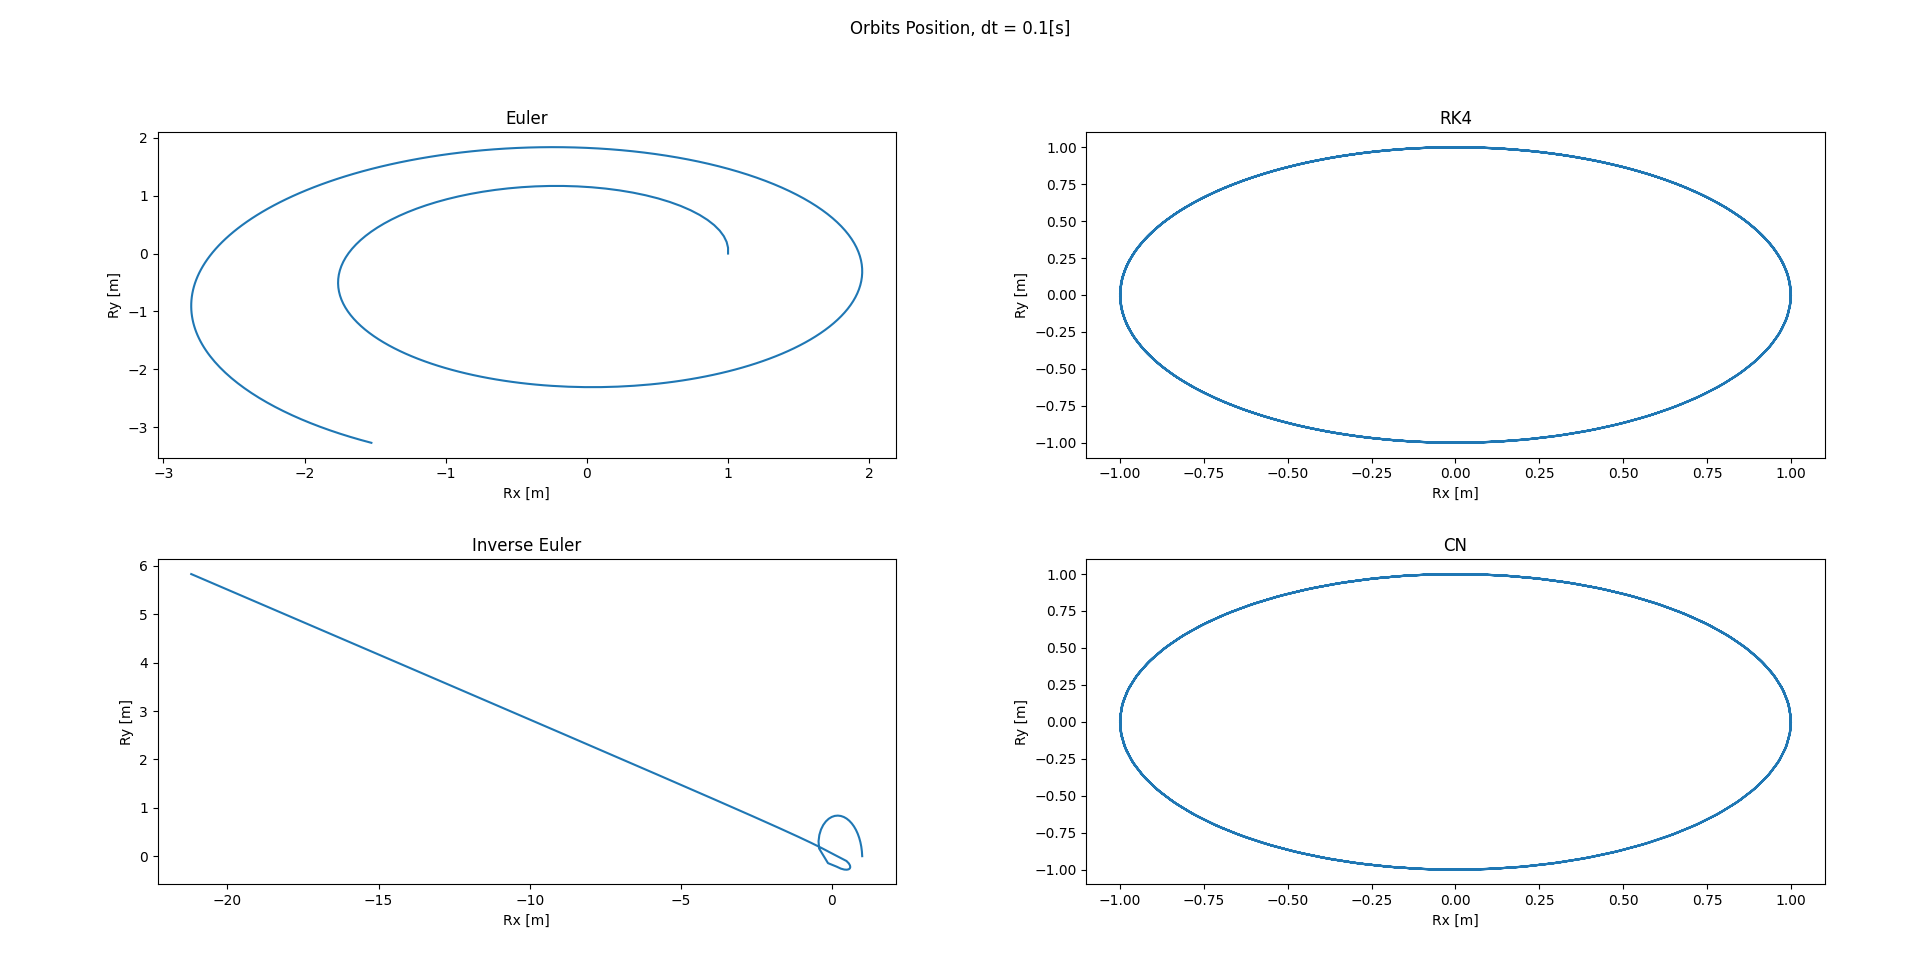
\includegraphics[width=0.95\textwidth]{FIGURES/dt0.1_newton_pos.png}
	\caption{Resolución órbita de Kepler por varios métodos durante 30$s$.}
\end{figure}
\begin{figure}[H] 
	\centering
	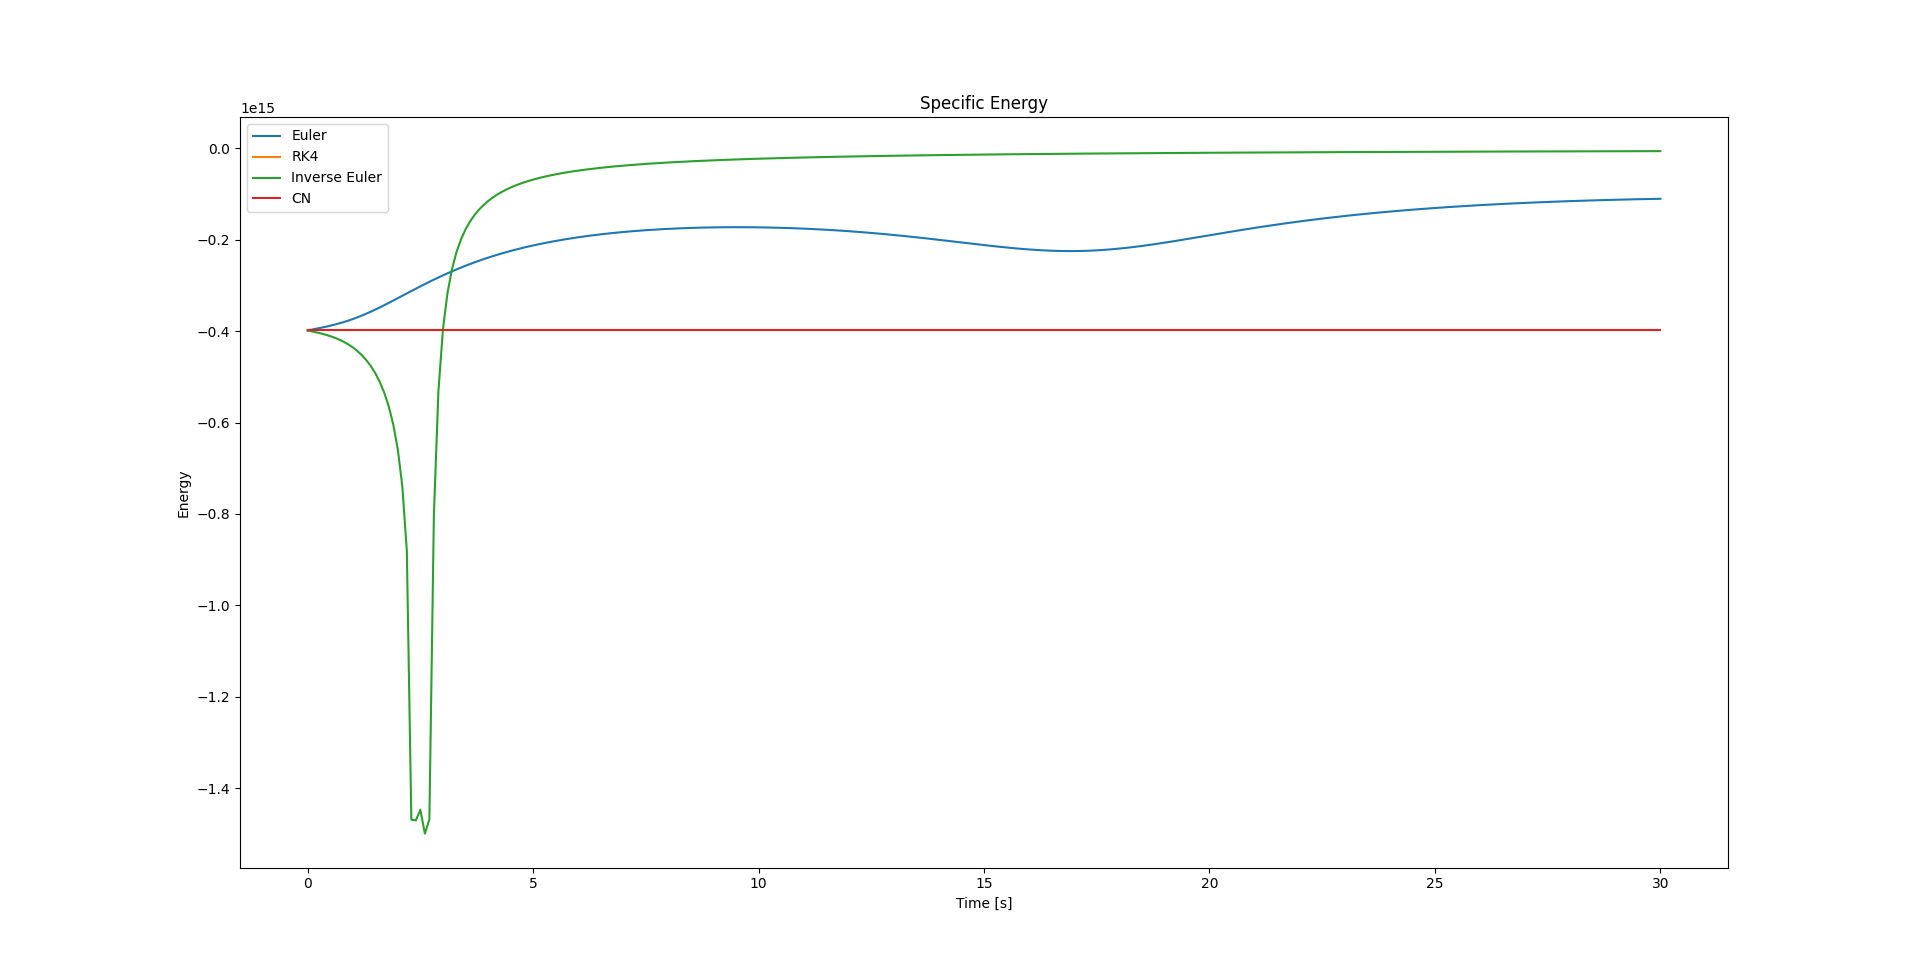
\includegraphics[width=0.95\textwidth]{FIGURES/dt0.1_fsolve_energy.png}
	\caption{Energía específica con $\Delta t = 0.1 s$.}
\end{figure}


\subsection{Simulaciones con: $\Delta t = 0.001 s$}

\begin{comment}
\begin{figure}[H] 
	\centering
	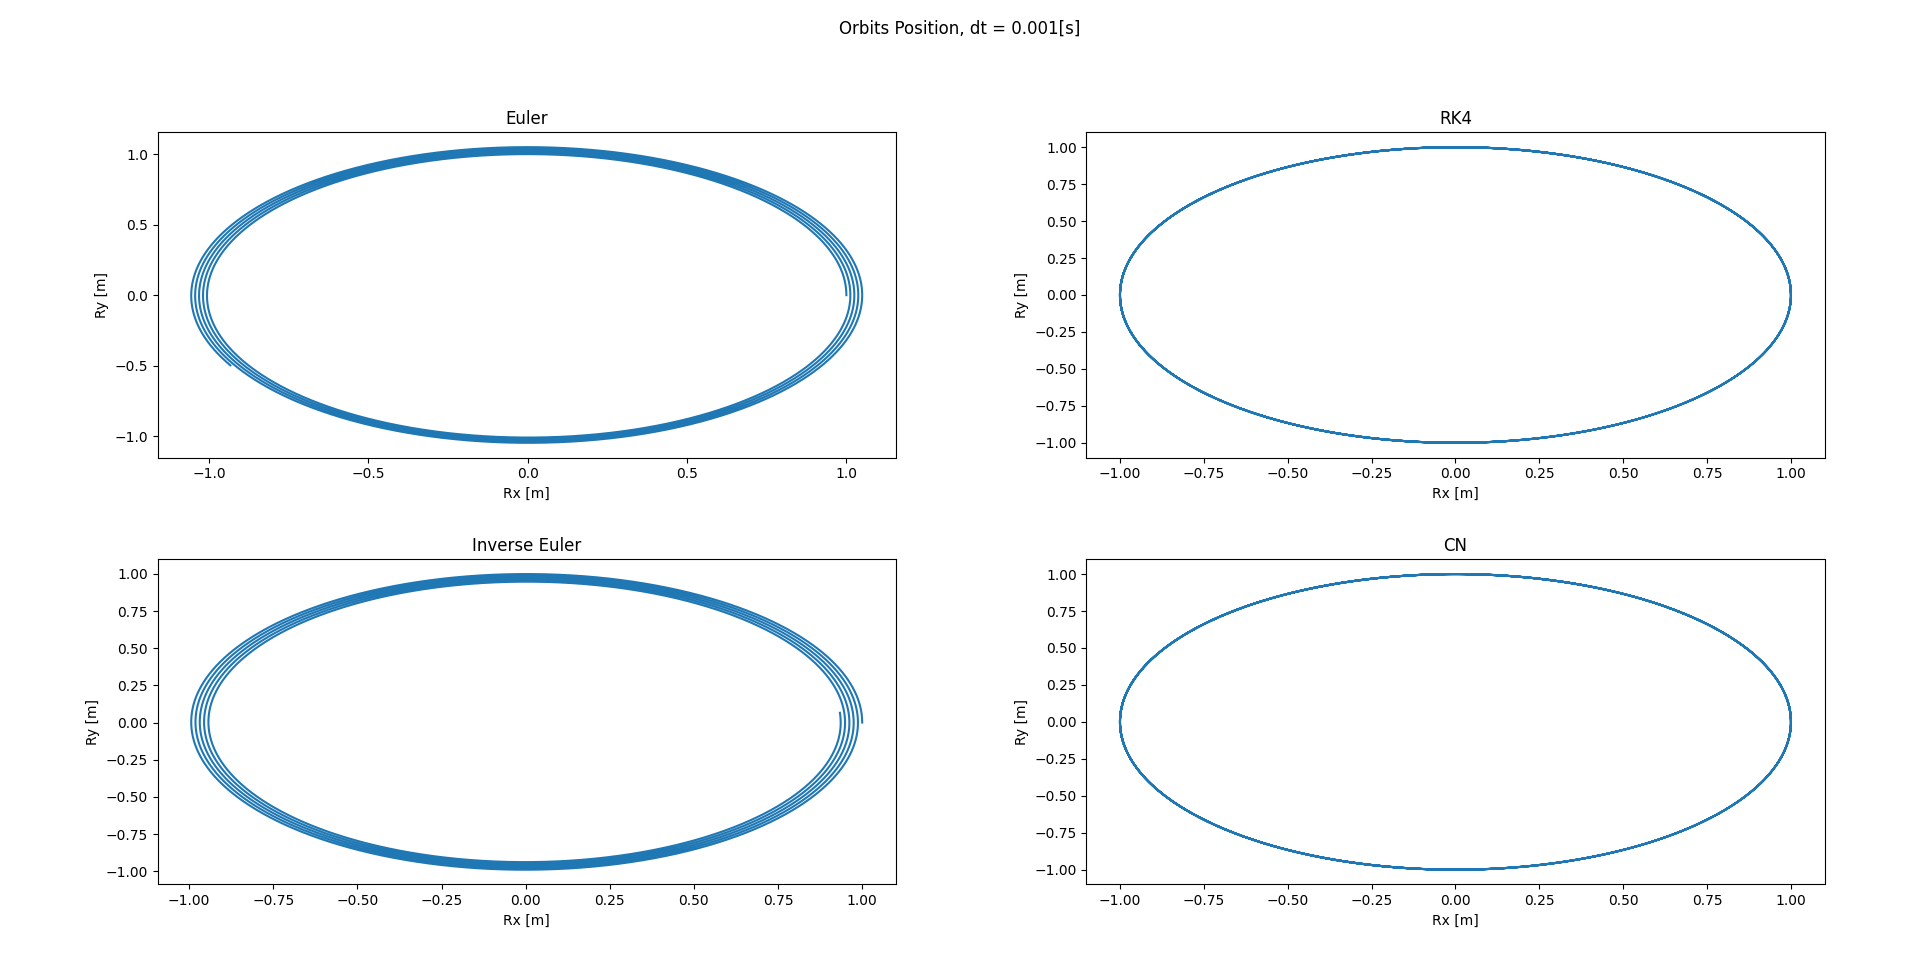
\includegraphics[width=0.95\textwidth]{FIGURES/dt0.001_fsolve_pos.png}
	\caption{Resolución órbita de Kepler por varios métodos durante 30$s$, utilizando $fsolve$.}
\end{figure}
\begin{figure}[H] 
	\centering
	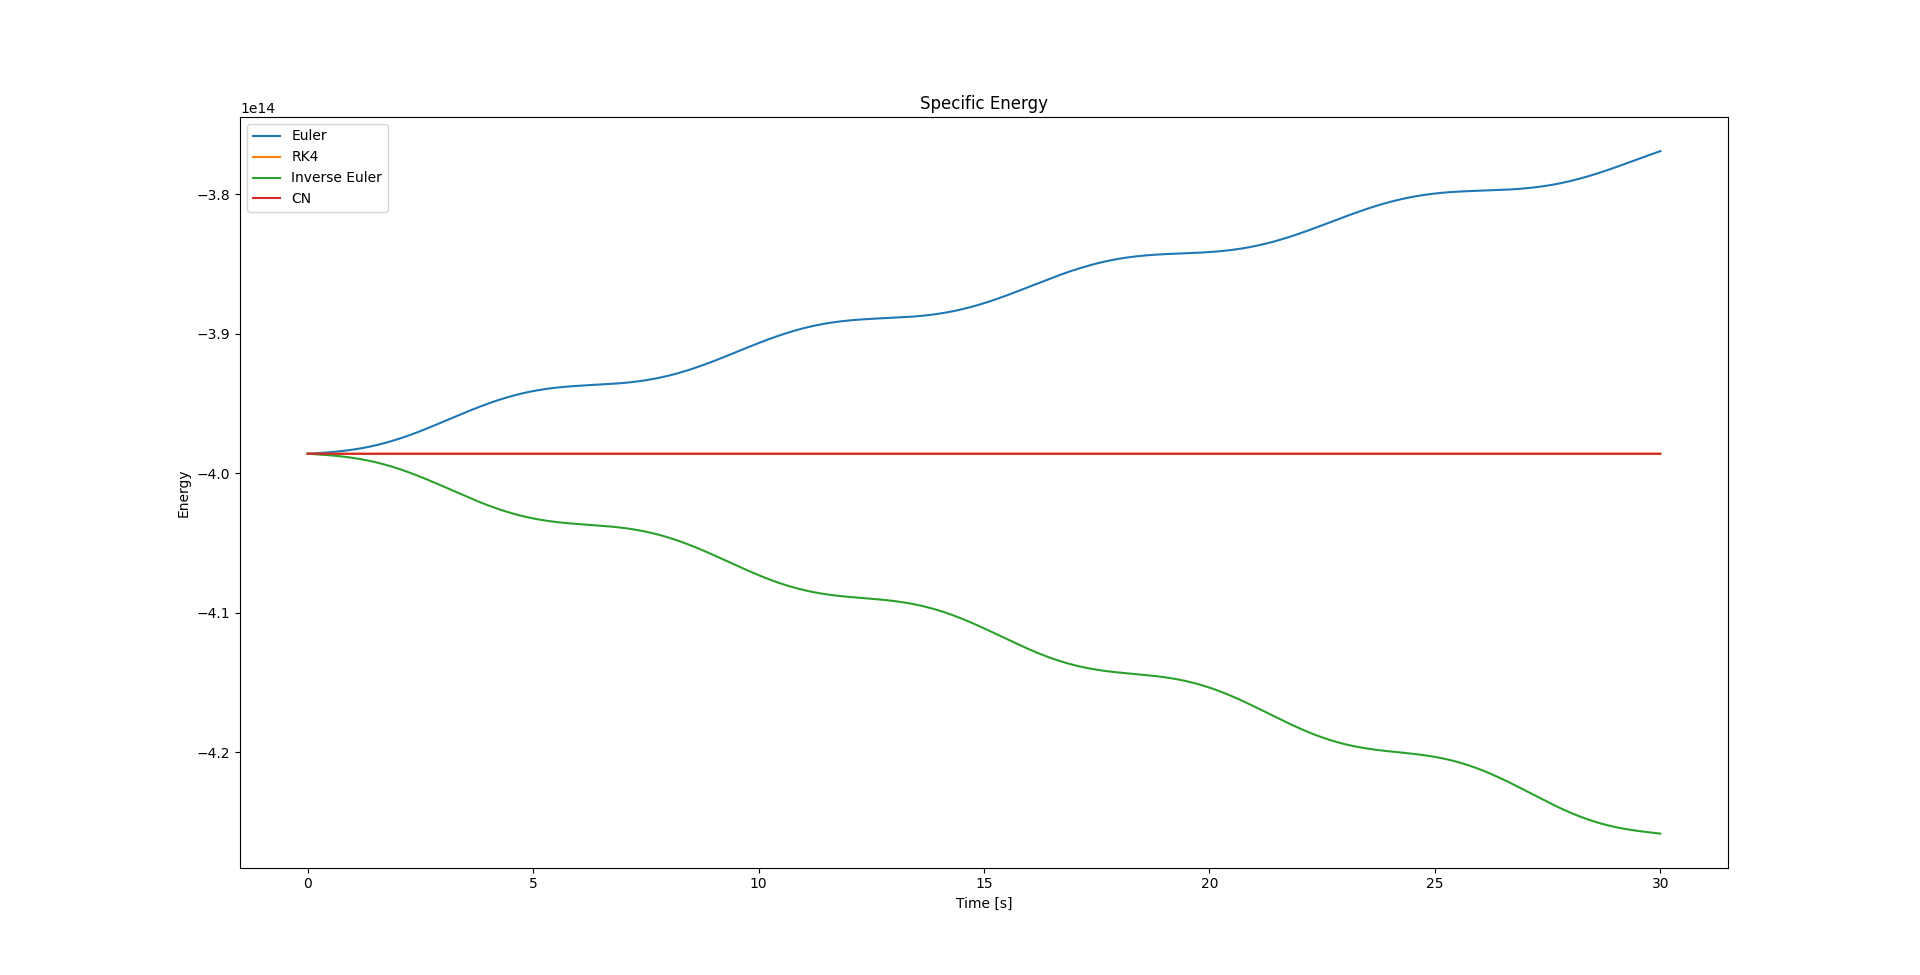
\includegraphics[width=0.95\textwidth]{FIGURES/dt0.001_fsolve_energy.png}
	\caption{Energía específica con $\Delta t = 0.001 s$, utilizando $fsolve$.}
\end{figure}
\end{comment}

Al disminuir el intervalo de tiempo para realizar el cálculo numérico se obtienen resultados con menor error. Los métodos de Runge-Kutta de orden 4 y de Crank-Nicolson mejoran aún su precisión. El método de Euler explícito reduce el error, así como el método inverso de Euler hace lo mismo. 
\begin{figure}[H] 
	\centering
	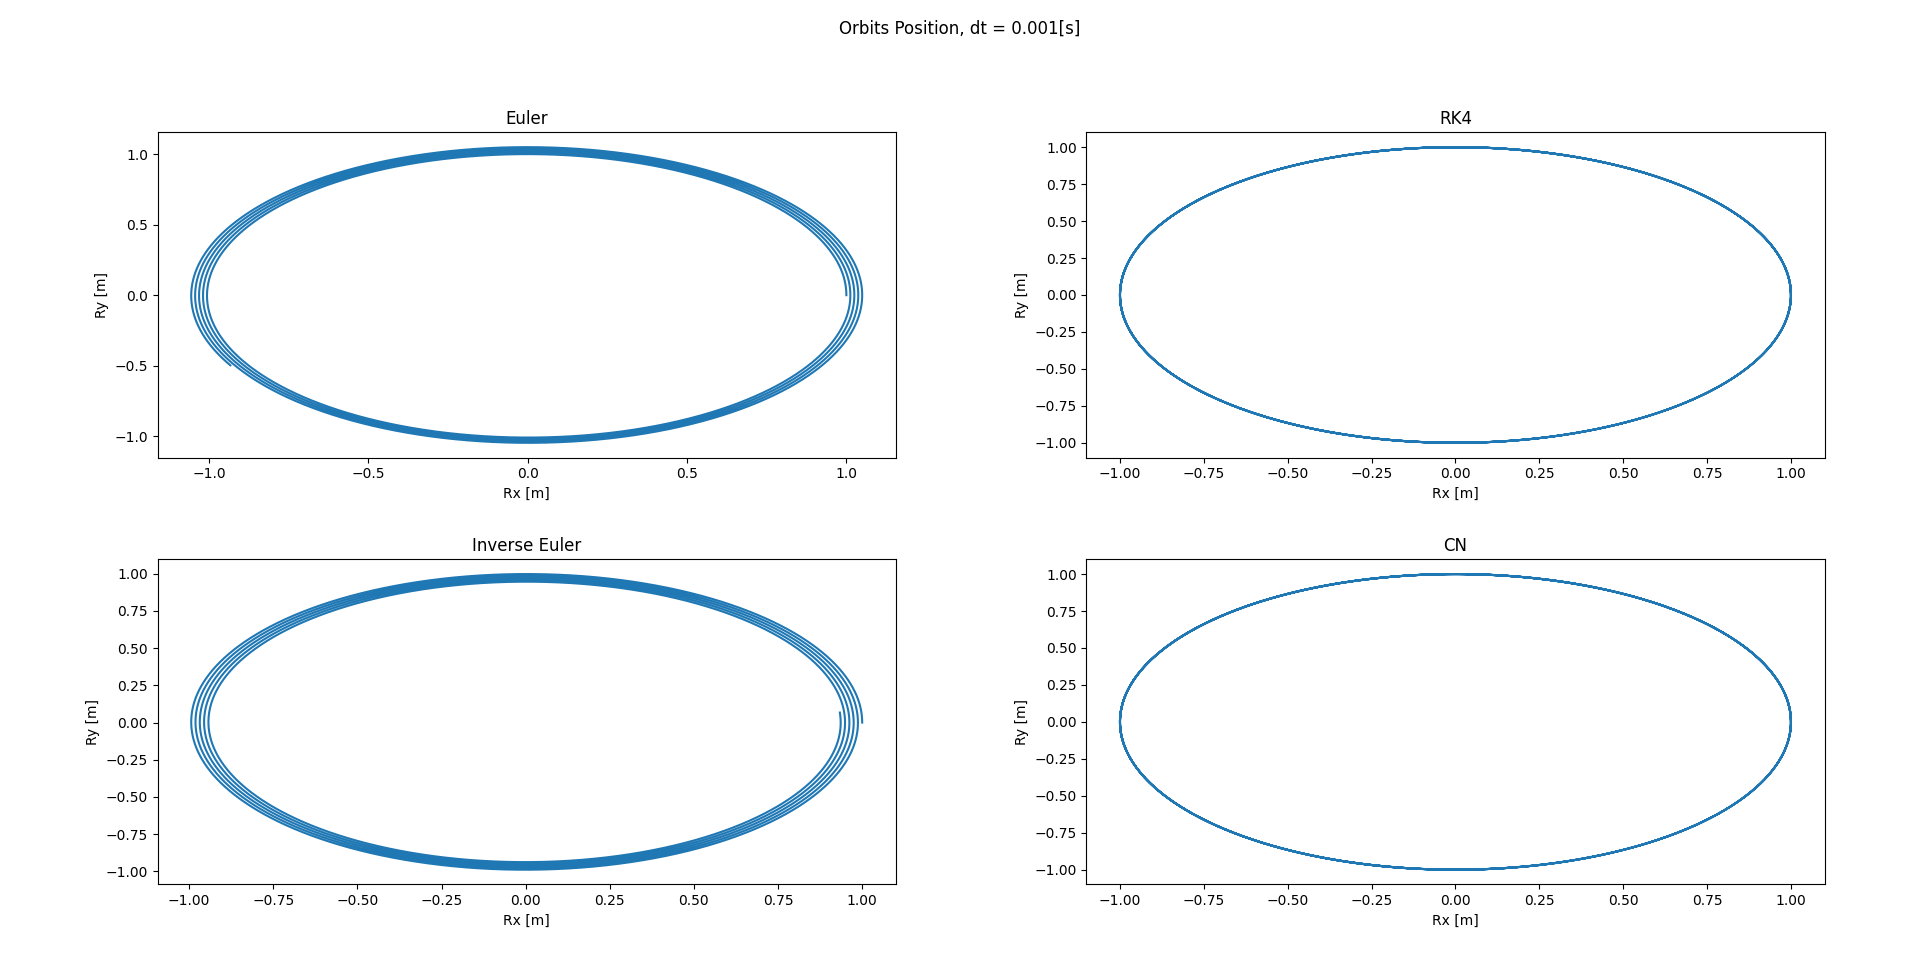
\includegraphics[width=0.95\textwidth]{FIGURES/dt0.001_newton_pos.png}
	\caption{Resolución órbita de Kepler por varios métodos durante 30$s$.}
\end{figure}
Respecto al análisis de la energía específica de la órbita cabe destacar que con el método de Euler explícito se aumenta su valor casi de forma lineal según va pasando el tiempo de simulación. Ocurre lo contrario y de manera simétrica con el método inverso de Euler. 
\begin{figure}[H] 
	\centering
	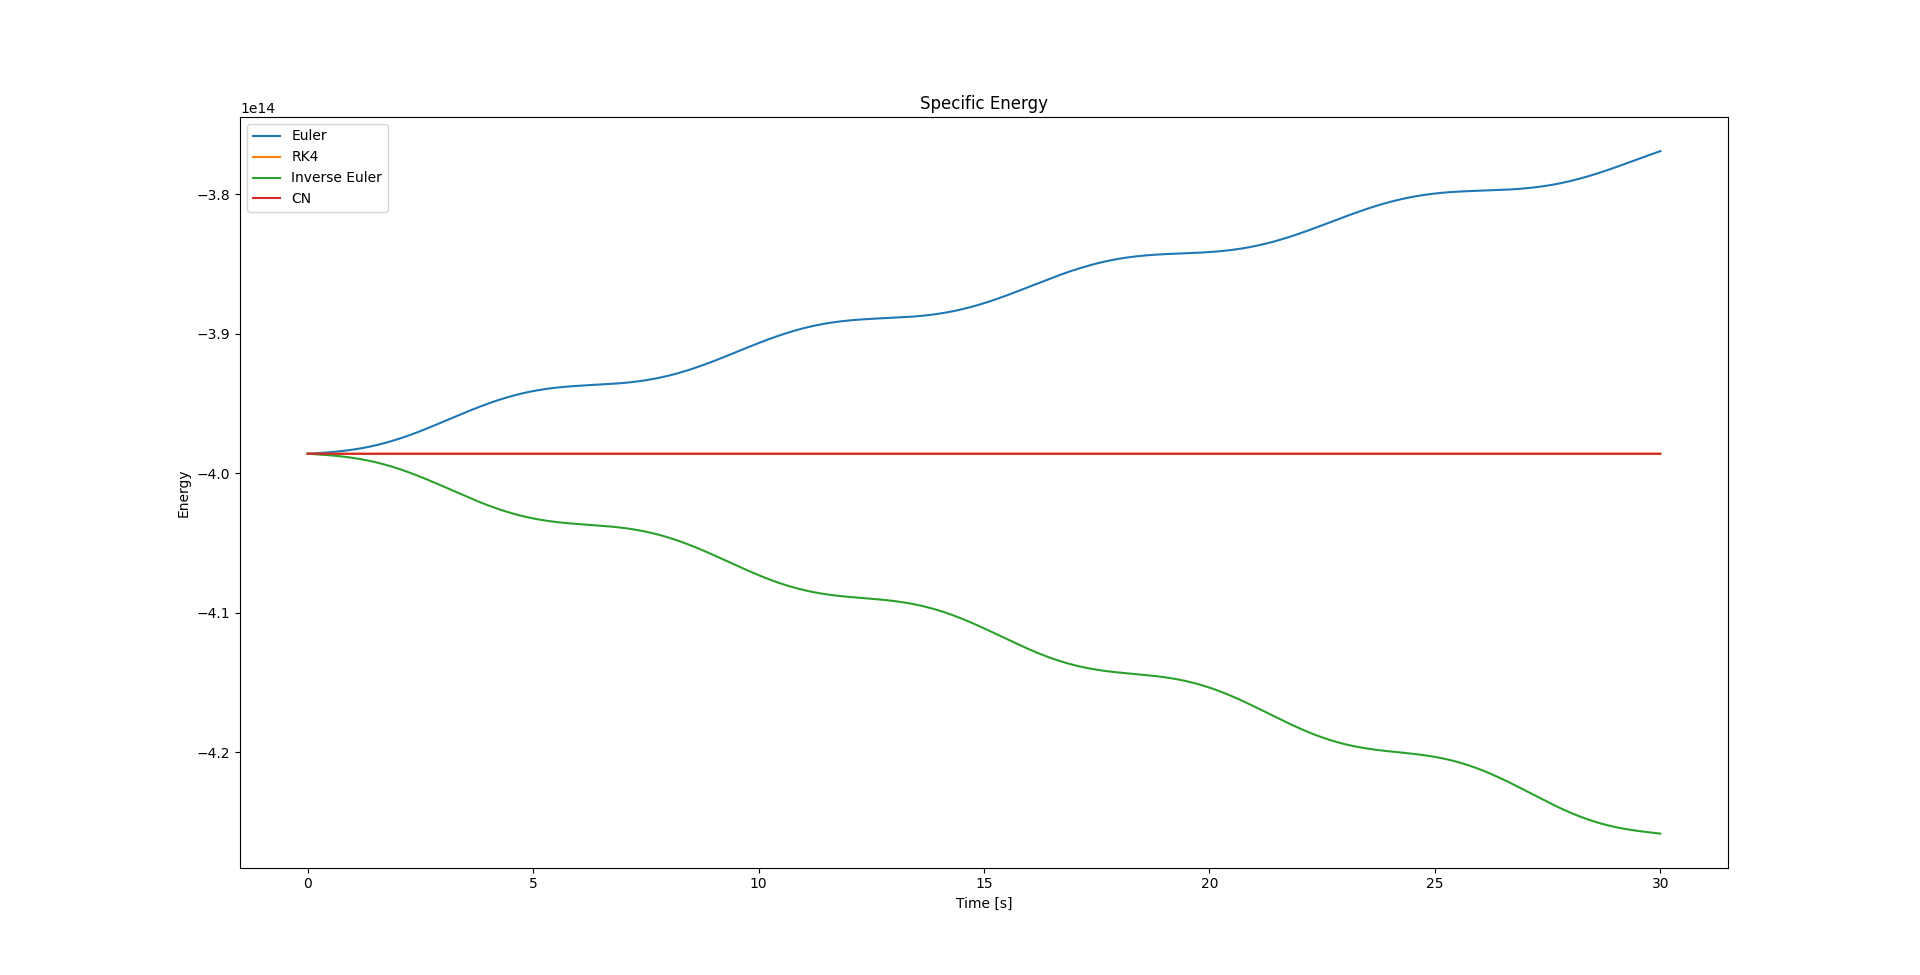
\includegraphics[width=0.95\textwidth]{FIGURES/dt0.001_fsolve_energy.png}
	\caption{Energía específica con $\Delta t = 0.001 s$.}
\end{figure}






\end{document}
